%
% File acl2021.tex
%
%% Based on the style files for EMNLP 2020, which were
%% Based on the style files for ACL 2020, which were
%% Based on the style files for ACL 2018, NAACL 2018/19, which were
%% Based on the style files for ACL-2015, with some improvements
%%  taken from the NAACL-2016 style
%% Based on the style files for ACL-2014, which were, in turn,
%% based on ACL-2013, ACL-2012, ACL-2011, ACL-2010, ACL-IJCNLP-2009,
%% EACL-2009, IJCNLP-2008...
%% Based on the style files for EACL 2006 by 
%%e.agirre@ehu.es or Sergi.Balari@uab.es
%% and that of ACL 08 by Joakim Nivre and Noah Smith

\documentclass[11pt,a4paper]{article}
\usepackage[hyperref]{acl2021}
\usepackage{times}
\usepackage{latexsym}
\usepackage{graphicx}
\renewcommand{\UrlFont}{\ttfamily\small}
\graphicspath{ {./images/} }

% This is not strictly necessary, and may be commented out,
% but it will improve the layout of the manuscript,
% and will typically save some space.
\usepackage{microtype}
\usepackage{booktabs}
\usepackage{float}


\aclfinalcopy % Uncomment this line for the final submission
%\def\aclpaperid{***} %  Enter the acl Paper ID here

%\setlength\titlebox{5cm}
% You can expand the titlebox if you need extra space
% to show all the authors. Please do not make the titlebox
% smaller than 5cm (the original size); we will check this
% in the camera-ready version and ask you to change it back.

\newcommand\BibTeX{B\textsc{ib}\TeX}

\title{Homework 1: Word-in-Context Disambiguation}

\author{Michele Conti \\
	\texttt{conti.1599133@studenti.uniroma1.it}\\}

\date{}

\begin{document}
	\maketitle
	\section{Introduction}
	WiC disambiguation is a binary classification task. Each instance in the dataset has a certain target word $w$ and two contexts (i.e., sentences) $c_1$ and $c_2$ in which $w$ is contained. The task is to identify whether the occurrences of the target word $w$ in the two sentences carry the same meaning or not.
	
	In this paper I present two architectures to address this task, both based on the use of pretrained embeddings and bilinear layers.

	\section{Preprocessing}	
	Various options have been considered in order to preprocess the data, but, ultimately, I decided to follow a very basic pipeline in this phase. Specifically, all the pairs of sentences have been lowercased, all the punctuation has been stripped, and finally I removed all the stopwords and digits from the sentences. As for stemming and lemmatization, instead, I specifically decided to avoid these operations for two reasons: the first one being that I already had in mind to exploit pretrained word embeddings, which are often computed for non lemmatized/stemmed words, and also because I felt like the specific form of each word could help disambiguate one sentence from the other.
	
	To create the vocabulary, it was my first decision to retain all the words appearing in the training dataset, no matter their frequency, since the training set is not very large (i.e., 26119 unique words after the preprocessing part).
	
	In the next sections we are going to see that even this step can be improved, creating the vocabulary from an external source. Specifically, I decided to inherit the vocabulary of Glove, an unsupervised learning algorithm for obtaining vector representations for words \citep{pennington2014glove}.

	\section{Models}
	\subsection{Models architecture}
	Two general structures have been used as baselines to assess the complexity of the given task, and to identify possible improvements in the models. Namely, the first structure I implemented is only based on linear layers, while the second one is composed by an LSTM followed by linear layers.
	
	
	\subsection{Embeddings}
	The very first module each architecture has is an embedding layer, where each token of each sentence gets projected into a vector space, so that the data can subsequently be fed to the next layers. This layer works as a lookup table between an index, indicating the position of the word in the vocabulary, and its vector representation, called embedding. The vector embeddings are randomly initialized, and they are then tuned during the training phase to minimize the loss function.
	
	\subsection{Embeddings aggregation}
	Once the embeddings for the words of both sentences are computed, we need a way to aggregate this information, to extract the meaning of the sentences as a whole. There are two general approaches we can use when trying to accomplish this task. The first one, the simplest, is to compute some summary statistic (e.g., sum, average, weighted average, etc.) of the set of embeddings. The second approach, on the other hand, involves the use of a recurrent layer to encode the sequence of embedding into a single vector.
	
	It's not always the case that harder is better: I noticed that, in this case, simple summary statistics works much better than sequence encoding. Specifically, taking the average of the embeddings seems to be the best option between the considered options (i.e., sum, average, weighted average centered around the target word).
	
	\subsection{Classification head}
	The embeddings aggregation is then linked to a classification head, which is composed of one linear layer and a ReLU activation function, followed by a final fully connected layer and a sigmoid function.

	\section{Experiments}
	In this section, we are going to explore possible modifications to these two baseline models we just described, comparing at each step the performance of the two structures.
	
	Since a wide range of features have been tested, at each step we're only going to keep the ones that proved to be effective, actually increasing the performance of the two models.
	
	All the variations here discussed have been trained using Adam \citep{kingma2017adam} as optimizer. Check table \ref{tab:MLP-model} and \ref{tab:LSTM-model} for details.
	
	\subsection{Pretrained word embeddings}
	The first and obvious feature I added to my models is to substitute randomly initialized word embeddings with pretrained ones. Pretrained word embeddings are in fact much more reliable than the ones we could train on our data, since they are trained on very large corpora and therefore allow very high generalization.
	
	Moreover, I noticed that training my own word embedding, my models couldn't even surpass a random classifier, thus the mandatory need of a different strategy.
	
	For this purpose, as I already anticipated in the preprocessing section, I used Glove, adopting its vocabulary as my own, and considering as OOV words the ones that didn't appear in it. For these words, I decided to use a randomly initialized vector as embedding.
	
	Using pretrained embeddings, the accuracy increased from 49.10\% to 65.50\% in the MLP model, and from 51.10\% to 63.60\% in the LSTM one.
	
	\subsection{Dropout layers}
	One of the main issues when dealing with the task of WiC disambiguation is the very high risk of overfitting. There is in fact a very big gap between training and validation accuracy, even after just a few epochs. For this reason, I decided to use Dropout layers \citep{JMLR:v15:srivastava14a} after each linear (and recurrent) layer in both models.
	
	Using dropout layers, the accuracy increased from 65.50\% to 66.10\% in the MLP model, and from 63.60\% to 63.70\% in the LSTM one.
	
	\subsection{Improving the LSTM}
	There are still a couple of things we can tweak in the LSTM network to improve its performance. The first one is to adopt a \textbf{Bi-LSTM} architecture, taking into consideration both left-to-right and right-to-left contexts of the sentences. The second thing is to \textbf{stack two LSTM layers} together. The combination of these two techniques proved to be effective, increasing the accuracy from 63.70\% to 65.10\%.
	
	 Instead, using only one of these two techniques, or stacking more than two recurrent layers, only worsened the performance of the model.
	
	\subsection{Bilinear layer}
	There is still one last step which can be (dramatically) improved: the concatenation between the embeddings summary of the first sentence and the embeddings summary of the second one. I found out that one clever way of replacing this step was to add a bilinear layer, taking in input the two summary embeddings and outputting one single vector.
	
	This was actually the step that increased the performance the most, going from 66.10\% to 70.70\% in the MLP model, and from 65.10\% to 65.70\% in the LSTM one.
	
	\subsection{POS tagging}
	An honorable mention goes to part-of-speech tagging. This process consists in marking every token of a sentence with its part of speech. In theory, this tool could help with our classification task, as it should at least provide some additional information about OOV words.
	
	In my specific case, I used a pretrained POS tagger, tagging each word of both sentences. These tags were then replaced by an index and fed to an embedding layer. However, in practice this strategy only worsened the performance of the models, and was therefore discarded.
	
	\section{Conclusion}
	Contrary to what I expected, the model that performed the best (fig. \ref{fig:architecture}) was the one exploiting the average to encode a sequence of embeddings. It is also showcased we can increase the performance of the aforementioned models just by replacing the concatenation operation with a bilinear layer.
	\clearpage
	\section{Figures and tables}
	All figures and tables have been intentionally placed at the end of the document, in this section, so that they don't affect the maximum limit of two pages for the text.
	\begin{figure}[H]
		\centering
		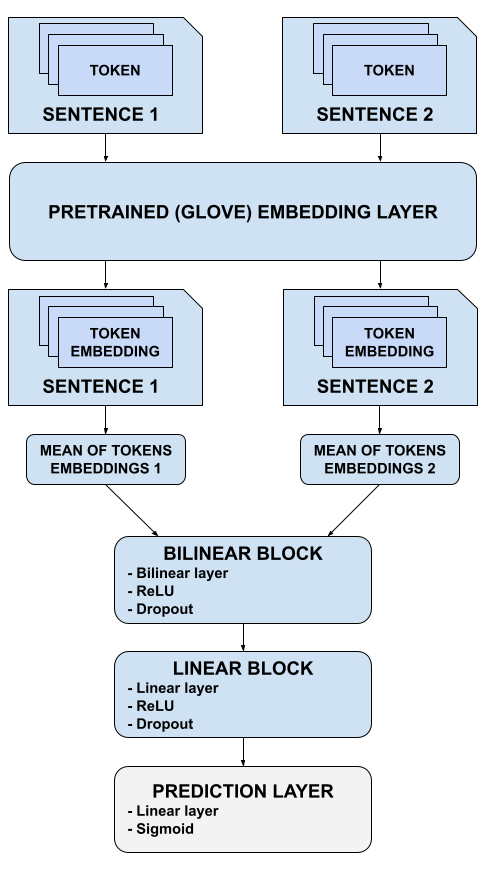
\includegraphics[width=1\columnwidth]{bilinear_model.png}
		\caption{Final model architecture.}
		\label{fig:architecture}
	\end{figure}

	\begin{table}[H]
		\centering
		\begin{tabular}{@{}ll@{}}
			\toprule
			\textbf{Model}               & \textbf{Accuracy (\%)} \\ \midrule
			MLP = Baseline MLP           & 49.10              \\
			MLP$_1$ = MLP + Glove*       & 65.50 (+ 16.4)     \\
			MLP$_2$ = MLP$_1$ + Dropout  & 66.10 (+ 0.6)      \\
			MLP$_3$ = MLP$_2$ + Bilinear & 70.70 (+ 4.6)     \\ \bottomrule
		\end{tabular}
		\caption{Performance gain of the MLP model, where MLP refers to the model that doesn't use an LSTM layer to encode the sequence of embeddings. The star operator * indicates the fact that a particular layer is pretrained.}
		\label{tab:MLP-model}
	\end{table}
	
	\begin{table}[H]
		\centering
		\begin{tabular}{@{}ll@{}}
			\toprule
			\textbf{Model}                                        & \textbf{Accuracy (\%)} \\ \midrule
			LSTM = Baseline LSTM                                  & 51.10                  \\
			LSTM$_1$ = LSTM + Glove*                              & 63.60 (+ 12.5)         \\
			LSTM$_2$ = LSTM$_1$ + Dropout                         & 63.70 (+ 0.1)          \\
			LSTM$_3$ = Bi-LSTM$_2$ + (stacked $\times$ 2) & 65.10 (+ 1.4)          \\
			LSTM$_4$ = LSTM$_4$ + Bilinear                        & 65.70 (+ 0.6)       \\ \bottomrule  
		\end{tabular}
		\caption{Performance gain of the LSTM model, where LSTM refers to the model that uses an LSTM layer to encode the sequence of embeddings. The star operator * indicates the fact that a particular layer is pretrained.}
		\label{tab:LSTM-model}
	\end{table}

	\begin{table}[H]
		\centering
		\begin{tabular}{@{}ll@{}}
			\toprule
			\textbf{Hyperparameter}  & \textbf{Value} \\ \midrule
			Batch size               & 64             \\
			Optimizer                & Adam           \\
			Learning rate            & 0.0001         \\
			Weight decay             & 0.0001         \\
			Embedding size           & 300            \\
			Embedding dropout        & 0              \\
			Bilinear hidden dim.     & 400            \\
			Linear hidden. dim       & 400            \\
			Bilinear \& linear dropout & 0.3            \\
			Activation function      & ReLU           \\ \bottomrule
		\end{tabular}
		\caption{Hyperparameters for the final model. All these parameters have been tested using a grid search and the results have been logged using Weight \& Biases.}
		\label{tab:hyperparameters}
	\end{table}
	
	\begin{figure}[H]
		\centering
		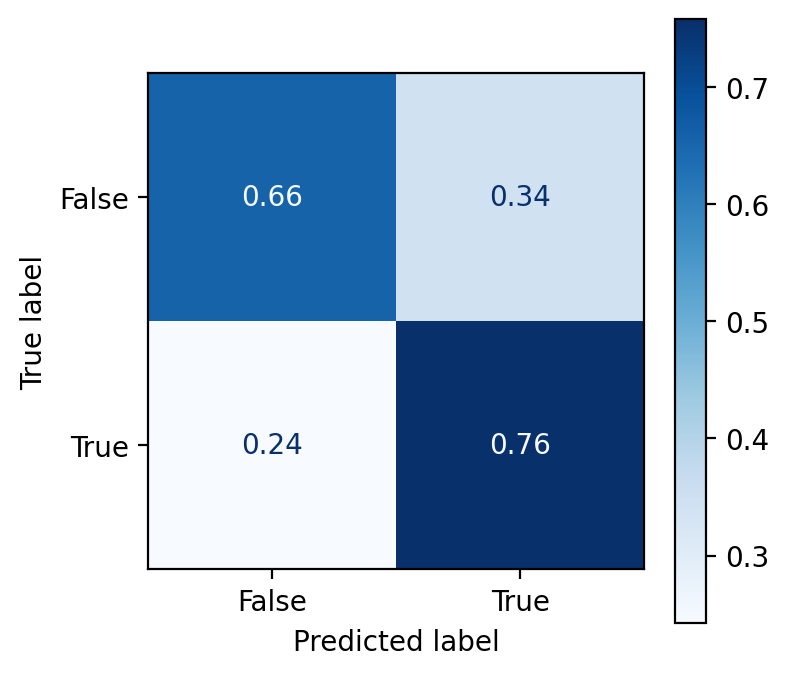
\includegraphics[width=1\columnwidth]{confusion_matrix.png}
		\caption{Normalized confusion matrix for the final model.}
		\label{fig:confusionmatrix}
	\end{figure}

	\begin{figure}[H]
		\centering
		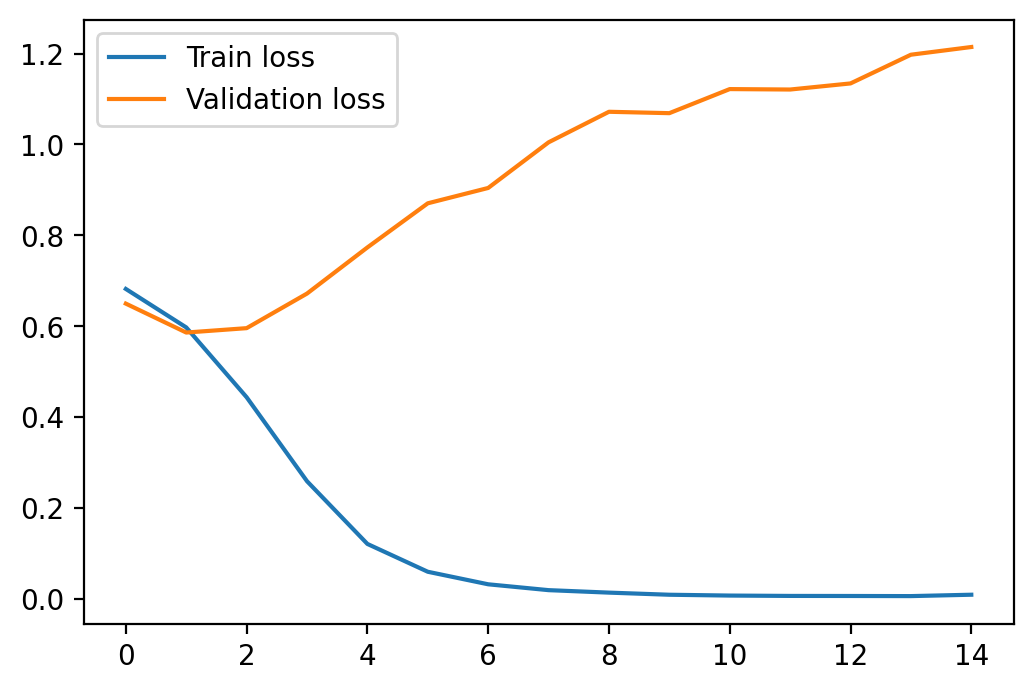
\includegraphics[width=1\columnwidth]{losses_final.png}
		\caption{Training and validation loss plot of the final model. This model obviously converges, and the validation loss starts to increase after very few epochs, when the model starts to overfit.}
		\label{fig:losses_final}
	\end{figure}

	\begin{figure}[H]
		\centering
		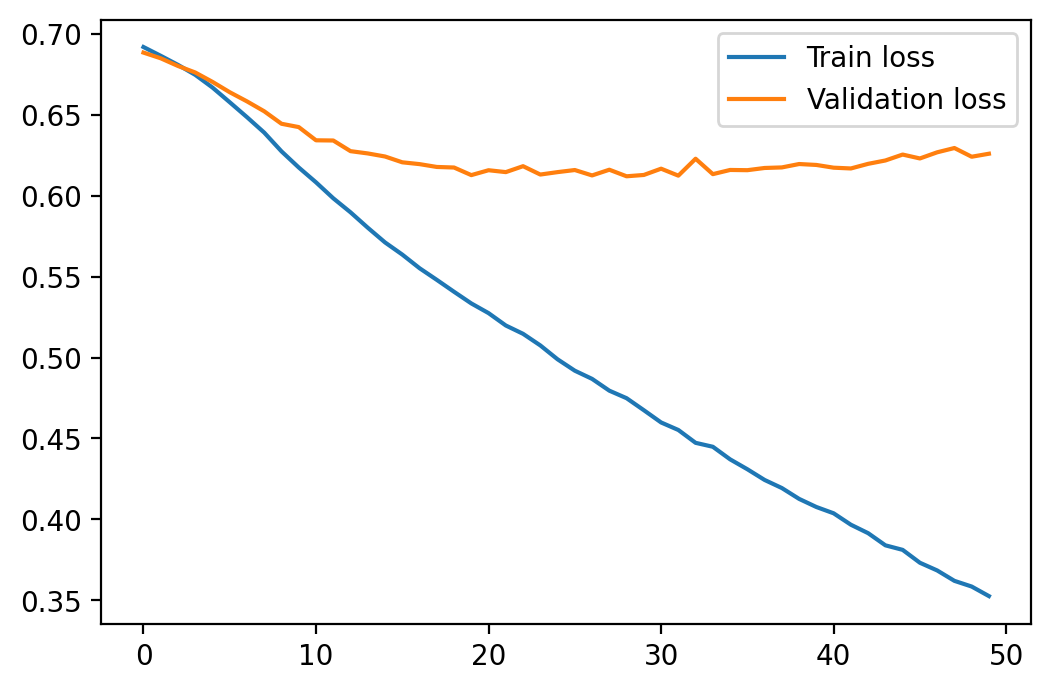
\includegraphics[width=1\columnwidth]{losses_mlp.png}
		\caption{Training and validation loss plot of the MLP$_3$ (i.e., last variation) model. This model never converges, which probably means that the concatenation of the sentence's embeddings is not the best way to handle the data.}
		\label{fig:losses_mlp}
	\end{figure}
	
	\bibliographystyle{acl_natbib}
	\bibliography{bibliography}
	
	%\appendix
	
	
	
\end{document}